% Drawing 138/06-15 -- folder 138, batch 06, archive page 113 (PDF page 114).
% Transcription: haut de page : une douzaine de petites cartes dessinées à l'encre, certaines entourées d'une courbe fermée portant un nombre ($8$, $9$, $6$) ; des faces marquées $1$, $3$, $4$, $5$ ; des chiffres $3$, $4$, $5$ écrits à côté, en partie surchargés ; un arbre, deux croix à quatre et trois branches ; des esquisses biffées.
% Kind: small maps (sheet of sketches). Method 2 (schematic redraw from the facsimile). Status: partial.
% Notes: Top of the page: small maps in ink, several surrounded by a closed curve carrying a number (8, 9, 6); faces marked 1, 3, 4, 5; numbers 3, 4, 5 written beside, partly overwritten; a tree, two crosses with four and three branches; struck sketches. Nine groups redrawn; vertex positions approximate, the doubled edge in the top-left map kept as two strokes, the overwritten numbers given as read (a « 3 » inside the lower-left map is overwritten) and the scribbles at the ends of the tree left out. Not encoded: these are sketches of maps whose faces and numbers are partly illegible.
% Coordinates: 1 unit = 1 mm = 1/100 of the crop width (bbox in page fractions: [0.12, 0.08, 0.92, 0.45]).
% Redrawn by Claude (claude-opus-5-5), issue #73, 2026-11-07; not checked by a human; not compiled (no TeX in the session).
% Rights: reproduces part of the work -- behind RENDER_TRANSCRIPTS, never published by itself.
\documentclass[tikz,border=3pt]{standalone}
\usepackage{amsmath,amssymb}
\usetikzlibrary{patterns,arrows.meta}
\tikzset{pencil/.style={black!45}, struck/.style={black!35}, mark/.style={circle,draw,inner sep=1.3pt}, pt/.style={circle,fill,inner sep=0.9pt}, opt/.style={circle,draw,fill=white,inner sep=1.1pt}}
\begin{document}
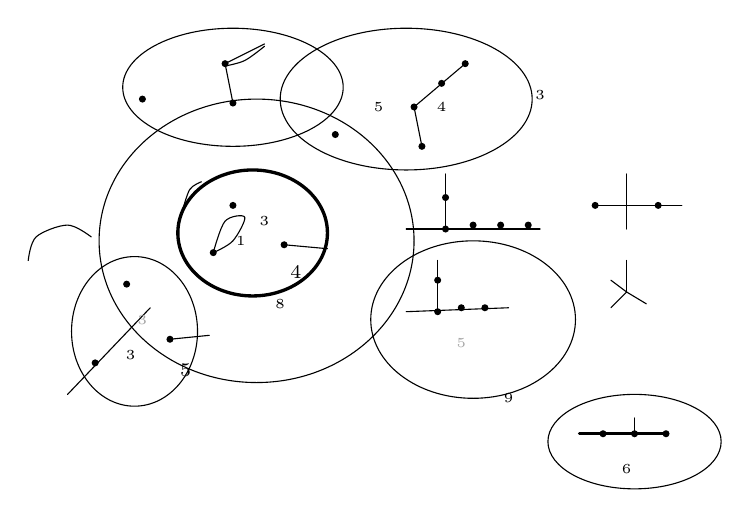
\begin{tikzpicture}[x=1mm,y=1mm,line cap=round,line join=round,font=\scriptsize]
\draw (29,-12) ellipse[x radius=14, y radius=7.5];
\draw (28,-9) -- (33,-6.5);
\draw plot[smooth, tension=0.55] coordinates {(28,-9.3) (30.5,-8.6) (33,-6.8)};
\draw (28,-9) -- (29,-14);
\node[pt] at (28,-9) {};
\node[pt] at (29,-14) {};
\node[pt] at (17.5,-13.5) {};
\draw (51,-13.5) ellipse[x radius=16, y radius=9];
\draw (52,-14.5) -- (58.5,-9);
\draw (52,-14.5) -- (53,-19.5);
\node[pt] at (42,-18) {};
\node[pt] at (52,-14.5) {};
\node[pt] at (55.5,-11.5) {};
\node[pt] at (58.5,-9) {};
\node[pt] at (53,-19.5) {};
\node[inner sep=1pt] at (47.5,-14.5) {\tiny $5$};
\node[inner sep=1pt] at (55.5,-14.5) {\tiny $4$};
\node[inner sep=1pt] at (68,-13) {\tiny $3$};
\draw (32,-31.5) ellipse[x radius=20, y radius=18];
\node[inner sep=1pt] at (35,-39.5) {\tiny $8$};
\draw[very thick] (31.5,-30.5) ellipse[x radius=9.5, y radius=8];
\draw plot[smooth, tension=0.55] coordinates {(26.5,-33) (28,-29) (30.5,-28.5) (29,-31.5) (26.5,-33)};
\draw (35.5,-32) -- (41,-32.5);
\node[pt] at (29,-27) {};
\node[pt] at (26.5,-33) {};
\node[pt] at (35.5,-32) {};
\node[inner sep=1pt] at (33,-29) {\tiny $3$};
\node[inner sep=1pt] at (30,-31.5) {\tiny $1$};
\node[inner sep=1pt] at (37,-35.5) {\scriptsize $4$};
\draw plot[smooth, tension=0.55] coordinates {(22.5,-28) (23.5,-25) (25,-24)};
\draw plot[smooth, tension=0.55] coordinates {(3,-34) (4,-31) (8,-29.5) (11,-31)};
\draw (16.5,-43) ellipse[x radius=8, y radius=9.5];
\draw (8,-51) -- (18.5,-40);
\draw (21,-44) -- (26,-43.5);
\node[pt] at (15.5,-37) {};
\node[pt] at (11.5,-47) {};
\node[pt] at (21,-44) {};
\node[inner sep=1pt,struck] at (17.5,-41.5) {\tiny $3$};
\node[inner sep=1pt] at (16,-46) {\tiny $3$};
\node[inner sep=1pt] at (23,-48) {\scriptsize $5$};
\draw (56,-23) -- (56,-30);
\draw (51,-30) -- (68,-30);
\node[pt] at (56,-26) {};
\node[pt] at (56,-30) {};
\node[pt] at (59.5,-29.5) {};
\node[pt] at (63,-29.5) {};
\node[pt] at (66.5,-29.5) {};
\draw (75,-27) -- (86,-27);
\draw (79,-23) -- (79,-30);
\node[pt] at (75,-27) {};
\node[pt] at (83,-27) {};
\draw (79,-38) -- (81.5,-39.5);
\draw (79,-34) -- (79,-38);
\draw (79,-38) -- (77,-36.5);
\draw (79,-38) -- (77,-40);
\draw (59.5,-41.5) ellipse[x radius=13, y radius=10];
\draw (55,-34) -- (55,-40.5);
\draw (51,-40.5) -- (64,-40);
\node[pt] at (55,-36.5) {};
\node[pt] at (55,-40.5) {};
\node[pt] at (58,-40) {};
\node[pt] at (61,-40) {};
\node[inner sep=1pt,struck] at (58,-44.5) {\tiny $5$};
\node[inner sep=1pt] at (64,-51.5) {\tiny $9$};
\draw (80,-57) ellipse[x radius=11, y radius=6];
\draw[very thick] (73,-56) -- (84,-56);
\draw (80,-54) -- (80,-56);
\node[pt] at (76,-56) {};
\node[pt] at (80,-56) {};
\node[pt] at (84,-56) {};
\node[inner sep=1pt] at (79,-60.5) {\tiny $6$};
\end{tikzpicture}
\end{document}
